\section{Strategy}


O padrão Strategy define grupos de algoritmos encapsulados e
intercambiáveis para um determinado contexto. Esses 
algoritmos podem ser definidos ou trocados em tempo de 
execução, permitindo que os clientes que os utilizem possam
alternar entre as implementações definidas livremente.

O Strategy soluciona o problema de classes relacionadas 
diferirem apenas em algum comportamento, permitindo que 
esse comportamento possa ser isolado e o resto da implementação 
das classes reaproveitado. Ele também evita a utilização de 
muitas operações condicionais. Ao invés de verificar qual 
deve ser o comportamento toda vez que ele precisar ser 
executado, o comportamento é pré-definido pelo contexto. 

A estrutura do padrão pode ser vista na figura \ref{strategy_struct}, 
onde uma interface é responsável por definir que operações 
uma estratégia deve possuir, enquanto diversas classes 
concretas implementam essas operações definindo suas 
estratégias. A classe cliente é responsável por manter 
uma referência para a estratégia e chamar as 
operações desejadas.

\begin{figure}[htb]
	\caption{\label{strategy_struct}Estrutura do Strategy}
	\begin{center}
	    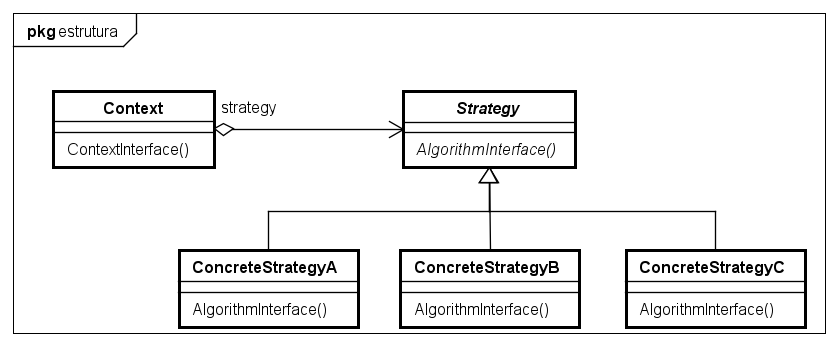
\includegraphics[scale=0.5]{5_padroes-contexto-funcional/5.3_comportamentais/5.3.09_strategy/strategy_estrutura.png}
	\end{center}
\end{figure}

\subsection*{Exemplo Orientado a Objetos}

O exemplo do Strategy apresenta uma \textit{stream} 
de texto que pode ser quebrada em linhas utilizando 
estratégias diferentes. A classe Composition 
gerencia as quebras de linha do texto exibidas em 
um editor, enquanto a interface Compositor define 
uma estratégia de quebra de linha. As estratégias 
apresentadas são representadas pelas classes 
SimpleCompositor, TeXCompositor e ArrayCompositor. 
A implementação desse exemplo pode ser vista no código 
\ref{oostrategy}, enquanto o diagrama de classes pode 
ser visto na figura \ref{strategy_exemplo}.

\begin{figure}[htb]
	\caption{\label{strategy_exemplo}Exemplo de Strategy}
	\begin{center}
	    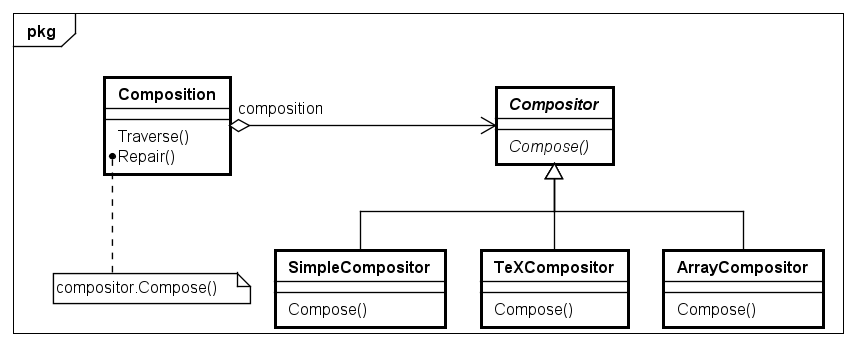
\includegraphics[scale=0.5]{5_padroes-contexto-funcional/5.3_comportamentais/5.3.09_strategy/strategy_exemplo.png}
	\end{center}
\end{figure}

\begin{lstlisting}[caption={Strategy Orientação a Objetos},label=oostrategy]
    
trait Compositor {
  def Compose(
             natural : Vector[Coord],
             stretch : Vector[Coord],
             shrink : Vector[Coord],
             componentCount : Int,
             lineWidth : Int,
             breaks : Vector[Coord]
             ) : Int
}

class SimpleCompositor extends Compositor {
  override def Compose(natural: Vector[Coord],
                       stretch: Vector[Coord],
                       shrink: Vector[Coord],
                       componentCount: Int,
                       lineWidth: Int,
                       breaks: Vector[Coord])
  : Int = {
    //Implementação do Simple Compositor
    0
  }
}

class TeXCompositor extends Compositor {
  override def Compose(natural: Vector[Coord],
                       stretch: Vector[Coord],
                       shrink: Vector[Coord],
                       componentCount: Int,
                       lineWidth: Int,
                       breaks: Vector[Coord])
  : Int = {
    //Implementação do TeX Compositor
    0
  }
}

class ArrayCompositor extends Compositor {
  override def Compose(natural: Vector[Coord],
                       stretch: Vector[Coord],
                       shrink: Vector[Coord],
                       componentCount: Int,
                       lineWidth: Int,
                       breaks: Vector[Coord])
  : Int = {
    //Implementação do Array Compositor
    0
  }
}

class Composition(var compositor: Compositor) {
  private var lineWidth : Int = 0
  private var lineBreaks : Vector[Coord] = Vector.empty
  private var lineCount : Int = 0

  def Repair() : Unit = {
    var natural = new Vector[Coord]
    var stretchability = new Vector[Coord]
    var shrinkability = new Vector[Coord]
    // Implementação da função repair
    val breakCount = compositor.Compose(
      natural, stretchability, shrinkability,
      lineCount, lineWidth, lineBreaks)
  }
}

\end{lstlisting}

\subsection*{Contexto Funcional}

Como a intenção do padrão é permitir a criação de 
grupos de algoritmos, ele é um candidato para o uso 
de funções de alta ordem. Ao invés de definir 
uma classe nova para cada implementação, a 
função Repair pode receber como parâmetro uma 
função compose que recebe como parâmetro um valor 
do tipo Compositor e retorna 
um inteiro. Dessa forma, basta definir as 
funções ComposeSimple, ComposeTeX e ComposeArray 
que podem ser passadas por parâmetro quando a 
função Repair for chamada. A implementação pode 
ser vista no código \ref{fpstrategy}.

\begin{lstlisting}[caption={Strategy Funcional},label=fpstrategy]
    
type Composition = (Int, List[Coord], Int)

type Compositor = (
    List[Coord],
      List[Coord],
      List[Coord],
      Int, Int,
      List[Coord])

def Repair(composition: Composition,
        compose : (Compositor) => Int): Unit = {
  var natural = List.empty
  var stretchability = List.empty
  var shrinkability = List.empty
  //Implementação da função Repair
  val breakCount = compose(
      (natural, stretchability, shrinkability,
     composition._3, composition._1, composition._2)
  )
}

def ComposeSimple(compositor : Compositor) : Int = {
  // implementação para SimpleCompositor
}

def ComposeTeX(compositor : Compositor) : Int = {
  // implementação para TeXCompositor
}

def ComposeArray(compositor : Compositor) : Int = {
  // implementação para ArrayCompositor
}
    
\end{lstlisting}

\begin{comment}
\subsection*{Vantagens e Desvantagens}

Utilizar funções de alta ordem no lugar do 
Strategy permite uma versatilidade maior quanto 
a que tipo de função pode ser aceita. Isso traz 
a vantagem de favorecer o reúso de funções que não 
foram planejadas para ser usadas como estratégias 
diferentes de implementação. Porém, traz a desvantagem 
de permitir que funções que possuam a mesma assinatura 
porém não realizem a operação desejada sejam passadas 
como estratégias válidas.
\end{comment}